\newcommand{\BrEquation}{
    \providecommand{\BrEqFontsize}{\fontsize{20pt}{20pt}\bf}
    \providecommand{\MatrixPadding}{-10pt}
    \begin{tikzpicture}
        \node (class_counts) at (0,0) {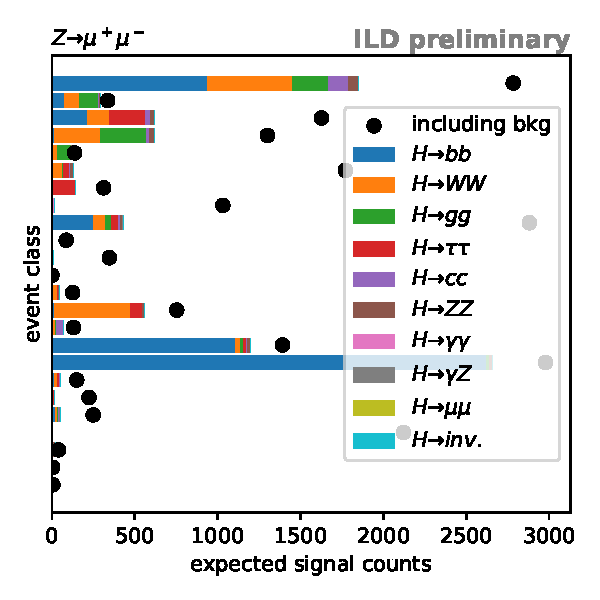
\includegraphics[width=2cm]{intro_category_counts_w_bkg}};
        \node[anchor=west] (eq) at (class_counts.east)  {\BrEqFontsize $=$};
        \node[anchor=west,xshift=\MatrixPadding] (matrix) at (eq.east)  {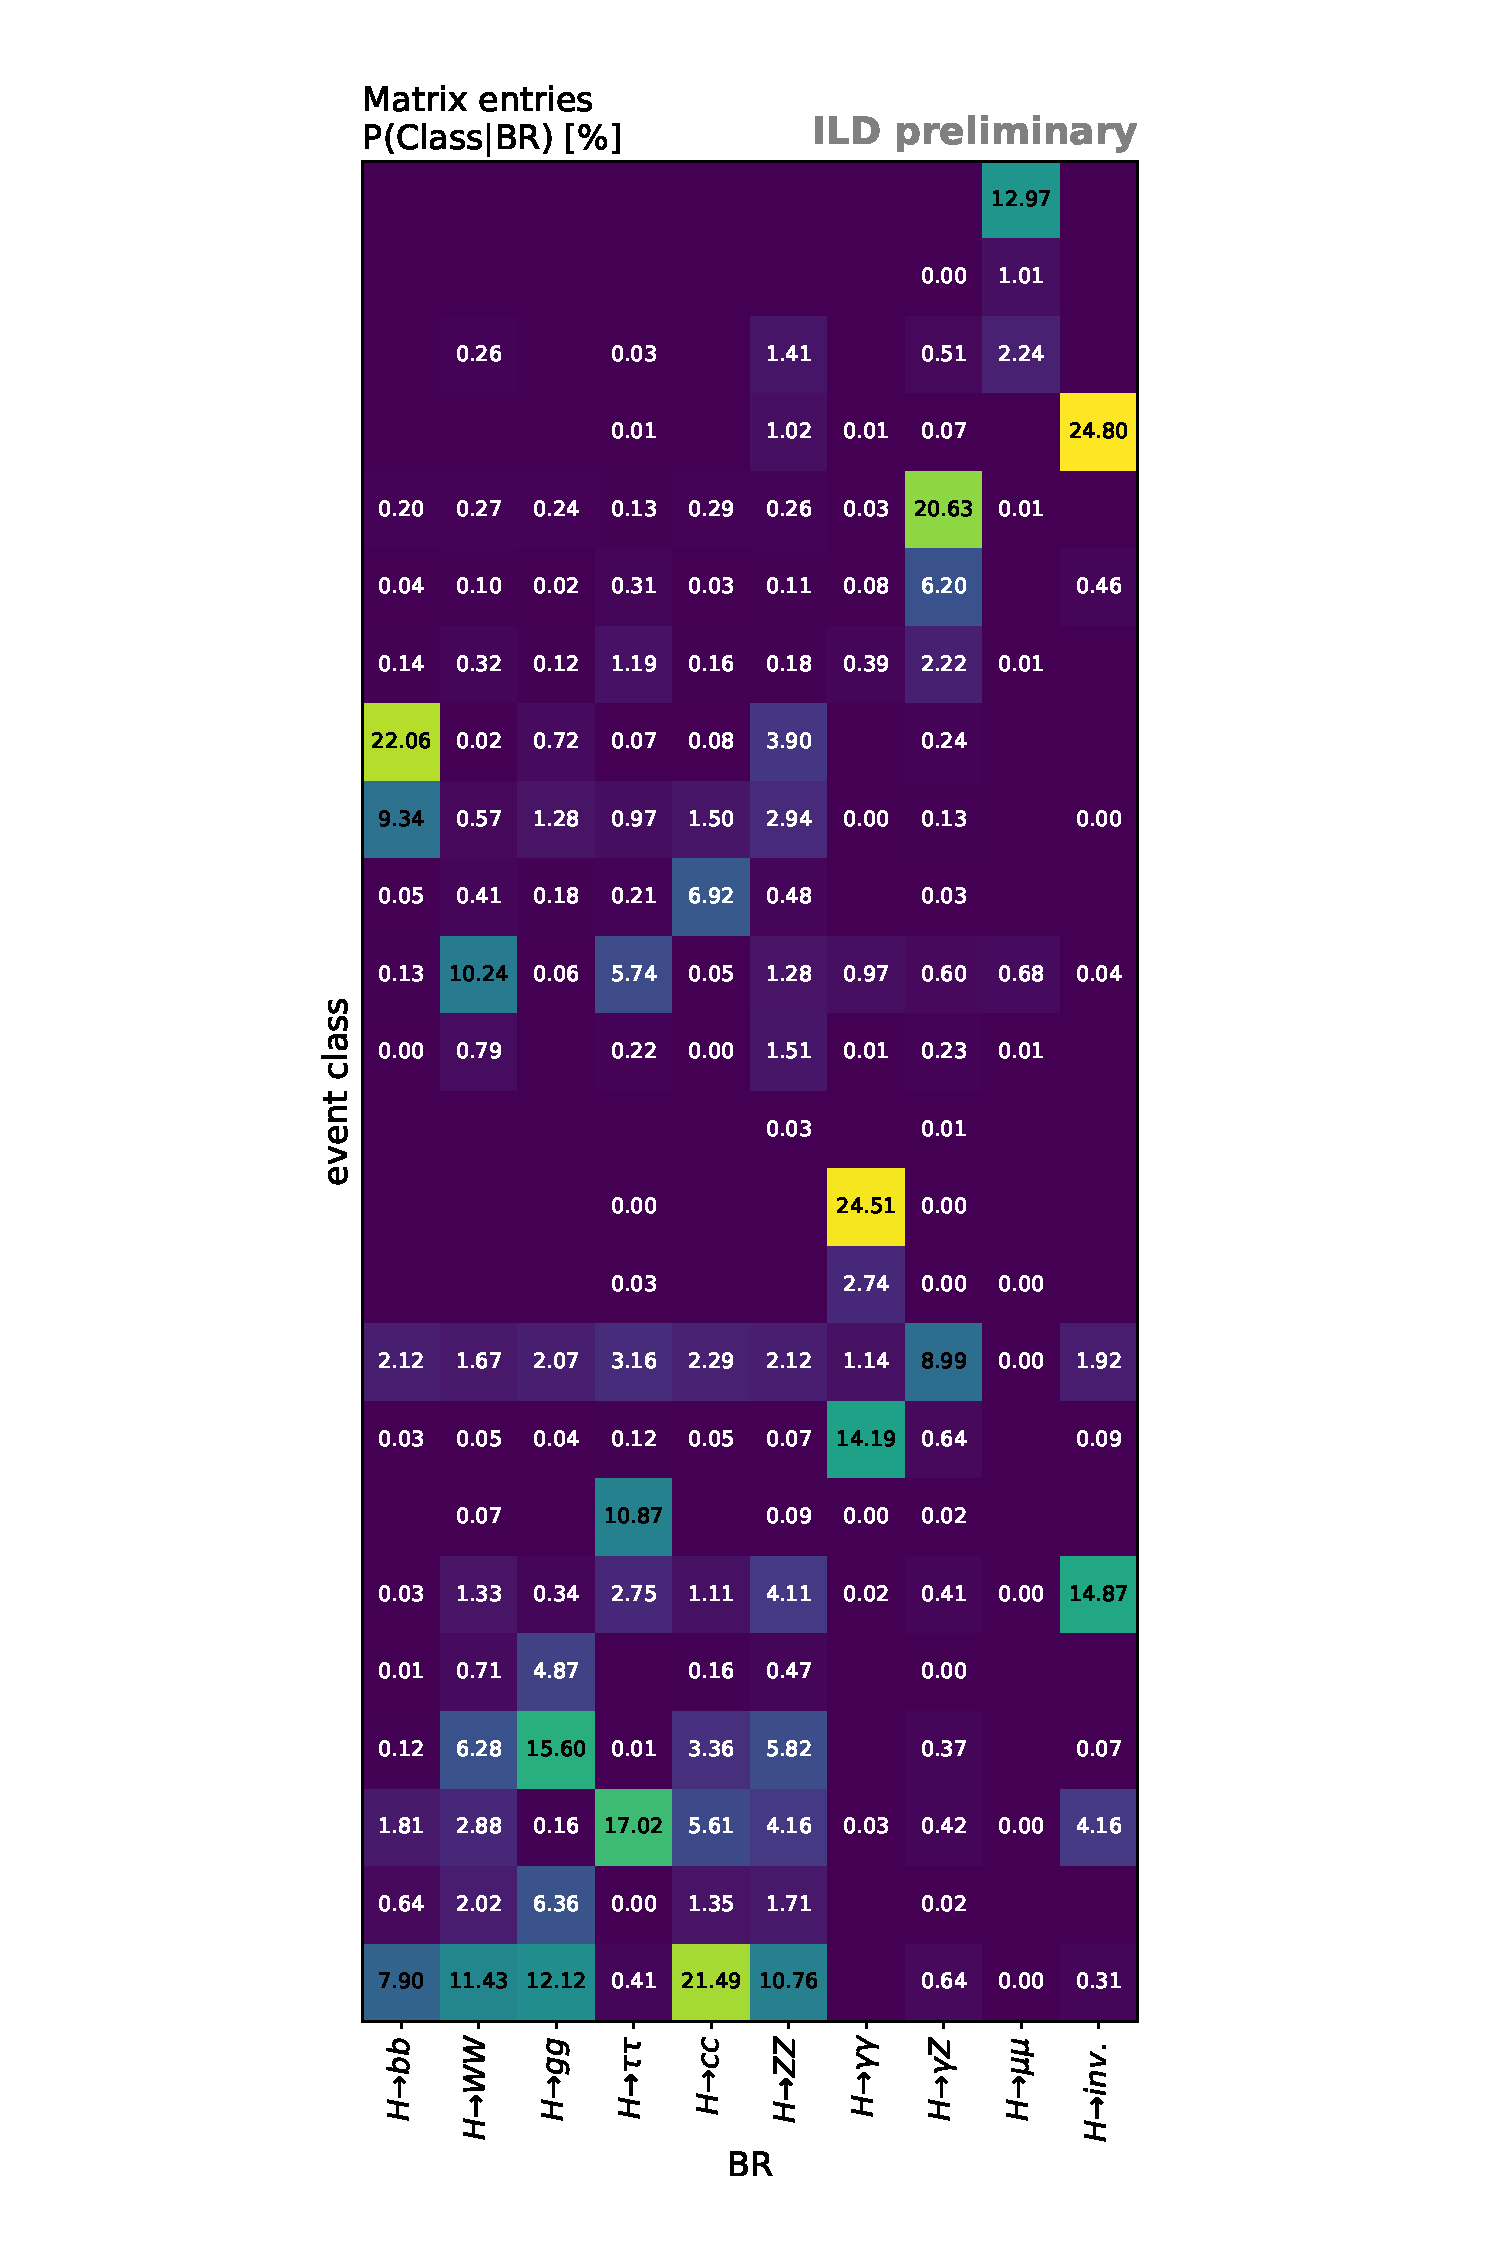
\includegraphics[width=2cm]{probability_matrix}};
        \node[anchor=west,xshift=\MatrixPadding] at (matrix.east) {\BrEqFontsize $\times~\mathcal{B}$};
    \end{tikzpicture}
}
\newcommand{\ColoredHiggsstrahlung}{
    \providecommand{\HiggsColor}{ILD_blue}\providecommand{\PrimaryZColor}{LLR_red}
    \resizebox{0.6\textheight}{!}{\FeynmanHiggsstrahlung}
}
\newcommand{\HiggsBlocks}[2]{
    \begin{columns}[b]
        \begin{column}{0.65\textwidth}#1\end{column}
        \begin{column}{0.35\textwidth}#2\end{column}
    \end{columns}
}
\begin{frame}
    \frametitle{Recap (1/2): Setup}
    %\renewcommand{\large}{\normalsize}\renewcommand{\normalsize}{\small} \normalsize
    \begin{columns}[onlytextwidth]
    \begin{column}{0.42\textwidth}\begin{minipage}[l][0.8\textheight]{\columnwidth}
        ILD full simulation study @ILC250.
        \vfill
        \begin{block}{\color{LLR_red}Event selection}\color{black}
            $Z \to \mu^+ \mu^-, e^+ e^-$.
            Cut-based. \\
            All Higgs decays, only uses the Z.
        \end{block}
        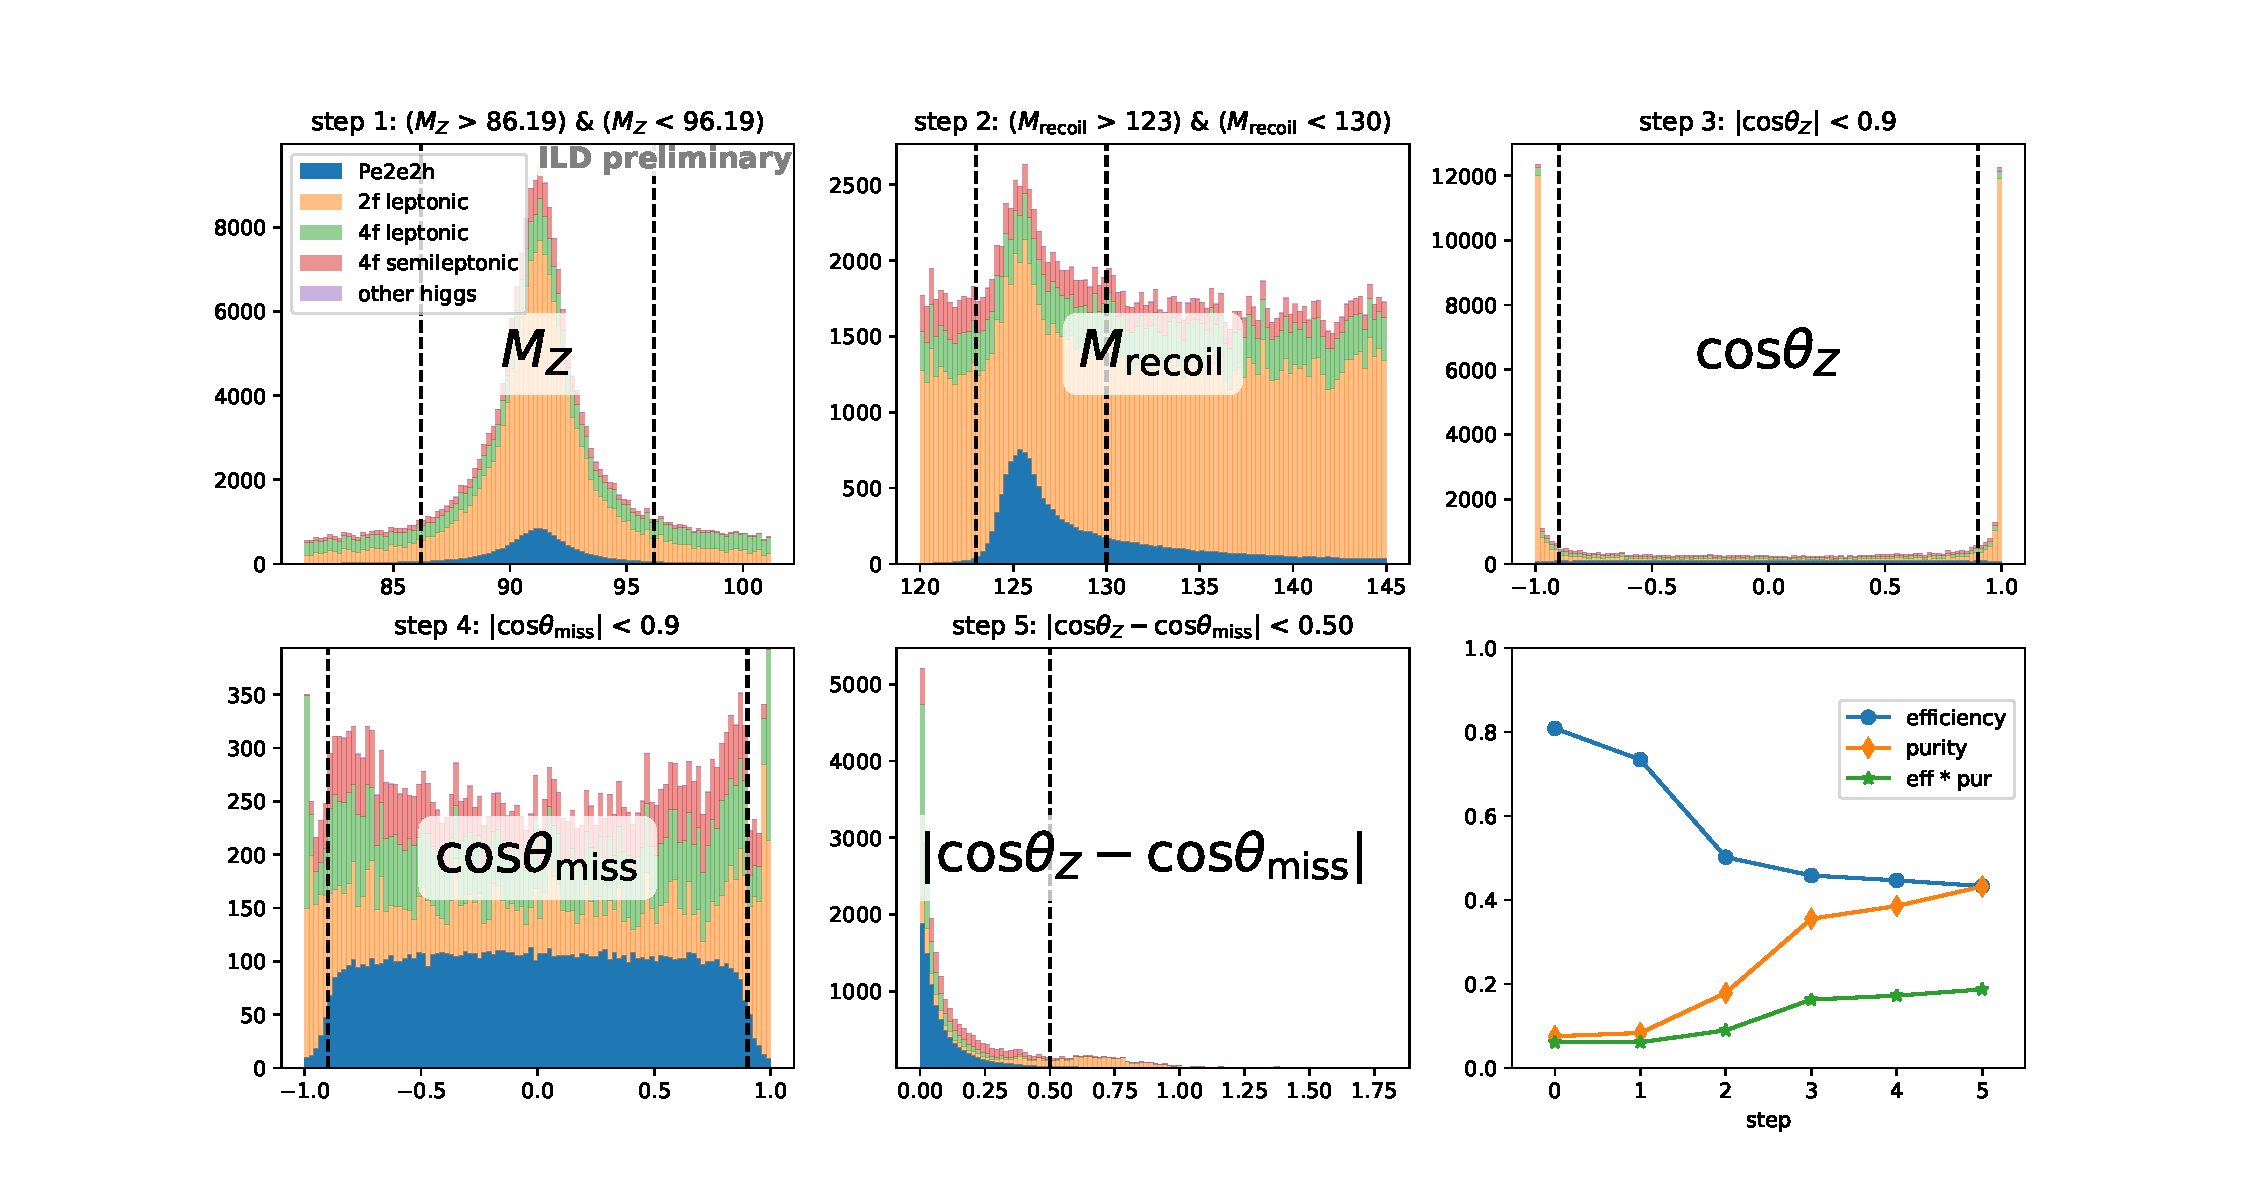
\includegraphics[width=0.9\textwidth]{presel_e2e2_for_proceedings}
    \end{minipage}\end{column}
    \begin{column}{0.58\textwidth}
    \HiggsBlocks{
        \ColoredHiggsstrahlung
        \begin{block}{\color{ILD_blue}Higgs classes}\color{black}
        Handcrafted.
        E.g. \textit{\small (btag1 > 0.9) \& (btag2 > 0.9) \& (no IsoLepton)}.
        \end{block}
    }{
        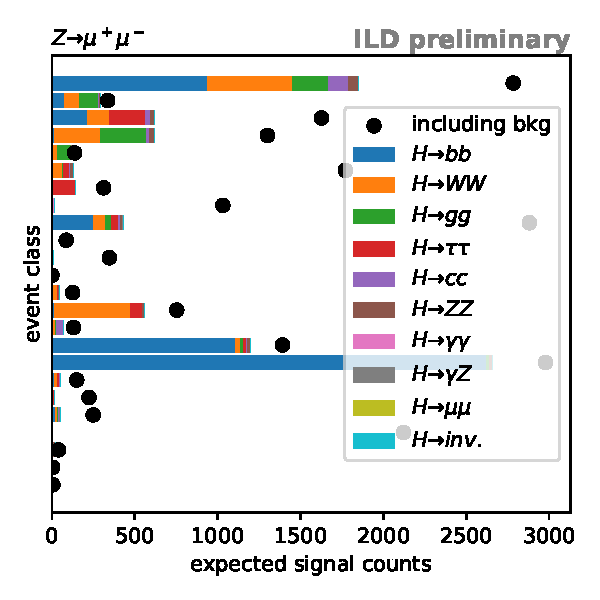
\includegraphics[width=\textwidth]{intro_category_counts_w_bkg}
    }
    \HiggsBlocks{
        \begin{block}{\color{black}Higgs BRs}\color{black}
        Obtain $\mathcal{B}$ and correlations from fit.
        Matrix from large MC samples per Higgs decay and background.
        \end{block}
    }{
        \resizebox{\textwidth}{!}{\BrEquation}
    }
    \end{column}
    \end{columns}
    \end{frame}


\begin{frame}{Recap (2/2): Results}
    \begin{columns}[c, onlytextwidth]
    \begin{column}{0.4\textwidth}
    \centering
    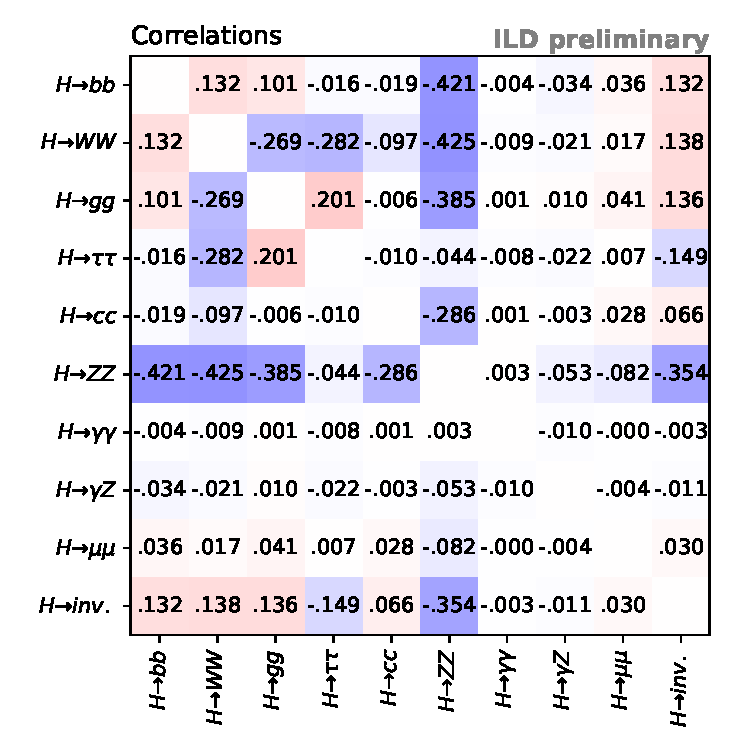
\includegraphics[height=0.7\textheight]
        {correlations_default}
    \end{column}
    \begin{column}{0.6\textwidth}
    \centering
    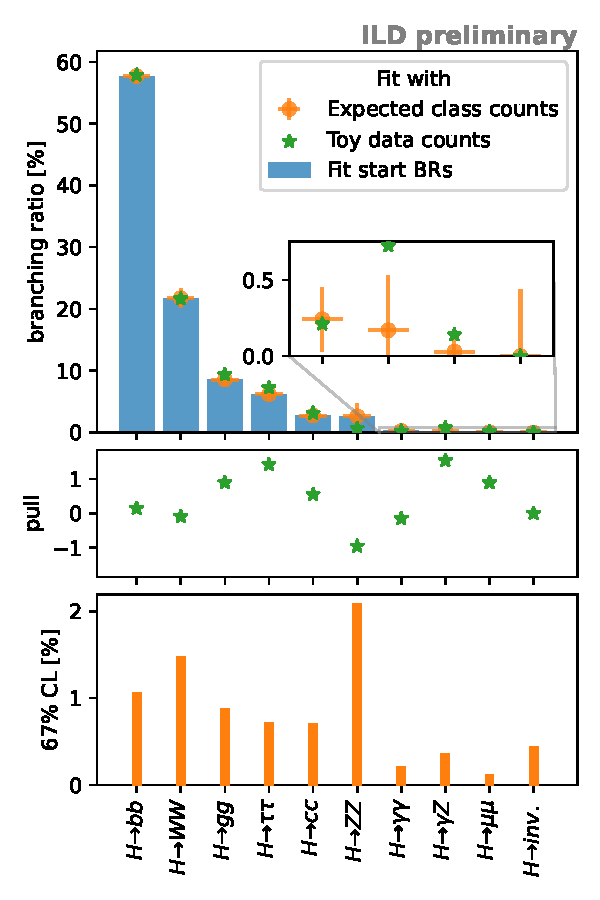
\includegraphics[height=0.9\textheight]{br_estimates_default}
    \end{column}
    \end{columns}
    \end{frame}
